%\pdfoutput=1 % only if pdf/png/jpg images are used
\documentclass{article}
\usepackage{amssymb}
%\usepackage[dvips]{graphicx}
\usepackage{graphicx}
\usepackage{verbatim}
\usepackage{xspace}
\newcommand{\E}{EIGER\xspace}  
\begin{document}

\title{\E - short manual}
\date{\today}
\maketitle

\section{Usage}

\subsection{Mandatory setup - Hardware}
A EIGER single module (500~kpixels) needs:
\begin{itemize}
\item A chilled (water+alcohol) at approximately 21~$^{\circ}$C, which needs to dissipate 85~W.
\item A power supply (12~V, 8~A).
\item 2$\times$1~Gb/s ethernet connectors to control the detector and, optionally, receive data at low rate. A DHCP server that gives IPs to the 1~Gb/s connectors of the detector is needed.
\item 2$\times$10~Gb/s transceivers to optionally, receive data at high rate.
 \end{itemize}

Figure~\ref{fig:1} shows the relationship between the \textbf{Client} (which sits on a beamline control PC), the \textbf{Receiver} (which can run in multiple instances on one or more PCs which receive data from the detector. The receiver(s) does not necessary have to be running on the same PC as the client.) It is important that the receiver is closely connected to the detector.

\begin{figure}[t]
\begin{center}
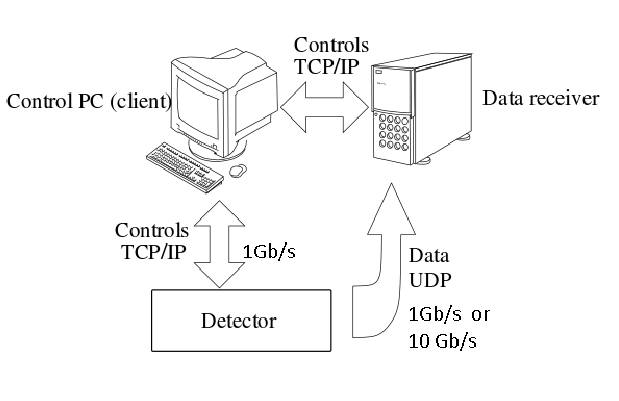
\includegraphics[width=.8\textwidth]{Client2}
\end{center}
\caption{Communications protocol between the Client PC, the receiver pc and the detector.}
\label{fig:1}
\end{figure}

The Client talks to control over 1~Gb ethernet connection using TCP/IP to the detector and to the receiver. The detector sends data in UDP packets to the receiver. This data sending can be done over 1~Gb/s or 10~Gb/s. 
 

\subsection{Mandatory setup - Receiver}

The receiver is a process run on a PC closely connected to the detector. Open one receiver for every half module board (remember, a module has two receivers!!!) . Go to {\tt{slsDetectorsPackage/bin/}}, \textbf{slsReceiver} should be started on the machine expected to receive the data from the detector.

\begin{itemize}
\item {\tt{./slsReceiver --rx\_tcpport xxxx}} 
\item {\tt{./slsReceiver --rx\_tcpport yyyy --mode 1}}
\end{itemize}

where xxxx, yyyy are the tcp port numbers. Use 1955 and 1956 for example. Note that {\tt{--mode 1}} is used only for the ``bottom'' half module. \\ Open as many receiver as half module boards. A single module has two half module boards.

\subsection{Mandatory setup - Client}

\underline{In the case of cSAXS, the detector software is installed on the x12sa-ed-1 machine:}\\
\underline{/sls/X12SA/data/x12saop/EigerPackage/slsDetectorsPackage}

The command line interface consists in these main functions:
\begin{description}
\item[sls\_detector\_acquire] to acquire data from the detector
\item[sls\_detector\_put] to set detector parameters
\item[sls\_detector\_get] to retrieve detector parameters
\end{description}


First, your detector should always be configured for each PC that you might want to use for controlling the detector. All the examples given here show the command {\tt{0-}}, which could be omitted for the EIGER system $0$. In the case more EIGER systems are controlled at once, the call of {\tt{1-}},.. becomes compulsory.

To make sure the shared memory is cleaned, before starting, one should do:  
\begin{verbatim}
sls_detector_get 0-free
\end{verbatim}
To do that:
\begin{verbatim}
sls_detector_put 0-config mydetector.config
\end{verbatim}
Refer to sample configuration files to produce the appropriate one for your detector.
\underline{In the case of cSAXS the {\tt{mydetector.config}} *at present* is:}\\ 
\underline{/sls/X12SA/data/x12saop/EigerPackage/beb\_1.5M\_1Gb\_fiber.config}

One can configure all the detector settings in a parameter file {\tt{setup.det}}, which is loaded by doing:
\begin{verbatim}
sls_detector_put 0-parameters setup.det
\end{verbatim}

In the case of \E, the proper bias voltage of the sensor has to be setup, i.e. the {\tt{setup.det}} file needs to contain the line {\tt{vhighvoltage 150}}. Other detector functionality, which are rarely changed can be setup here. 
Other important settings that are configured in the {\tt{setup.det}} file are:
\begin{itemize}
\item {\tt{tengiga 0/1}}, which sets whether the detector is enabled to send data through the 1~or the 10~Gb ethernet.
\item {\tt{flags parallel/nonparallel}}, which sets whether the detector is set in parallel acquisition and readout or in sequential mode. This changes the readout time of the chip and affects the frame rate capability (faster is {\tt{parallel}}, with higher noise but needed when the frame rate is $>2$~kHz. 
\item {\tt{dr 32/16}} sets the detector in autosumming mode (32 bit counter or not autosumming, 12 bit out of the chip). This is strictly connected to what is required for the readout clock of chip. See next point.
\item {\tt{clkdivider 0/1/2}}. Changes the readout clock: 200, 100, 50~MHz. Note that autosumming mode ({\tt{dr 32}} only works at {clkdivider 2}). By selecting Refer to readout timing specifications in~section\ref{timing} for how to set the detector. 
\item {\tt{flags continuous/storeinram}}. Allows to take frame continuously or storing them on memory. Normally {\tt{continuous}} should be used. Enabling the  {\tt{stroreinram}} mode allows you to obtain the maximum frame rate, but at the expenses to have to receive the data all at the end of the acquisition. Refer to readout timing specifications in section~\ref{timing} for how to set the detector.
\end{itemize}

One should notice that, by default, by choosing the option {\tt{dr 32}}, then the software automatically sets the detector to  {\tt{clkdivider 2}}. By choosing the option {\tt{dr 16}}, the software automatically sets the detector to  {\tt{clkdivider 1}}. One needs to choose {\tt{clkdivider 0}} after setting the {\tt{dr 16}} option to have the fastest frame rate. 
We would recommend expert users (beamline people) to write their parameters file for the users. 

\subsection{Standard acquisition}

You will then need to setup the detector threshold and settings, the exposure time, the number of real time frames and eventually how many real time frames should be acquired:
\begin{verbatim}
sls_detector_put 0-settings [standard/highgain/lowgain]
sls_detector_put 0-threshold 6000
sls_detector_put 0-exptime 1[time_is_s]
sls_detector_put 0-frames 10
sls_detector_put 0-period 0[time_is_s]
\end{verbatim}
In this case 10 consecutive 1~s frames will be acquired. Note that {\tt{period}} defines the sum of the acquisition time and the desired dead time before the next frame. If {\tt{period}} is set to 0, then the next frame will start as soon as the detector is ready to take another acquisition. \\

For \E, at the moment 3 settings are possible: {\tt{standard}}, {\tt{lowgain}} and {\tt{highgain}}. According to the setting chosen, one can reach different energies. Refer to the settings requirements for your detector.\\ 
Notice that the option  {\tt{settings standard/highgain/lowgain}} actually loads the trimbit files so it is time consuming. Only setting the {\tt{threshold}} does not load trimbit files.  

The threshold is expressed in (eV) as the proper threshold setting, i.e. normally is set to 50\% of the beam energy.  

\underline{At cSAXS, the {\tt{settingsdir}} and {\tt{caldir}} are in}\\\underline{/sls/X12SA/data/x12saop/EigerPackage/calibrations/}\\ 

You need to setup where the files will be written to
\begin{verbatim}
sls_detector_put 0-outdir /scratch
sls_detector_put 0-fname run
sls_detector_put 0-index 0
\end{verbatim}
this way your files will all be named /scratch/run\_dj\_i.raw where $j$ is relative to each specific half module, $i$ in the {\tt{index}} starts from 0 when starting the detector the first time and is automatically incremented. The next acquisition {\tt{index}} will be 1. One can reset the  {\tt{index}} to what wished.

To acquire simply type:
\begin{verbatim}
sls_detector_acquire 0-
\end{verbatim}

You can poll the detector status using:
\begin{verbatim}
sls_detector_get 0-status 
\end{verbatim}
If the receiver has not yet received the finished signal by the detector, the answer will return {\tt{running}}. If the detector has finished and ready for the next acquisition, then it will return {\tt{idle}}.
The detector will not accept other commands while acquiring. If an acquisition wishes to be properly aborted, then:
\begin{verbatim}
sls_detector_put 0-status stop 
\end{verbatim}
this same command can be used after a non proper abortion of the acquisition to reset to normal status the detector.

\subsection{Readout timing- maximum frame rate}\label{timing}
IMPORTANT: to have faster readout and smaller dead time, one can configure {\tt{clkdivider}}, i.e. the speed at which the data are read, i.e. 200/100/50~MHz for {\tt{clkdivider 0/1/2}} and the dead time between frames through {\tt{flags parallel}}, i.e. acquire and read at the same time or acquire and then read out.
The configuration of this timing variables allows to achieve different frame rates. NOTE THAT IN EIGER, WHATEVER YOU DO, THE FRAME RATE LIMITATIONS COME FROM THE NETWORK BOTTLENECK AS THE HARDWARE GOES FASTER THAN THE DATA OUT.

In the case of REAL CONTINUOUS readout, i.e. continuous acquire and readout from the boards (independent on how the chip is set):
\begin{itemize}
\item 1~GbE, {\tt{dr 16}}, {\tt{flags continous}}, \textbf{256~Hz} 
\item 1~GbE, {\tt{dr 32}}, {\tt{flags continous}}, {\tt{clkdivider 2}}, \textbf{128~Hz}
\item 10~GbE, {\tt{dr 16}}, {\tt{flags continous}}, {\tt{flags parallel}},{\tt{clkdivider 0}}, \textbf{2.56~kHz}  
\item 10~GbE, {\tt{dr 32}}, {\tt{flags continuous}}, {\tt{clkdivider 2}}, \textbf{1.28~kHz}  
\item 10~GbE, {\tt{dr 8}}, {\tt{flags continous}}, {\tt{flags parallel}},{\tt{clkdivider 0}}, \textbf{5.12~kHz}
\item 10~GbE, {\tt{dr 4}}, {\tt{flags continous}}, {\tt{flags parallel}},{\tt{clkdivider 0}}, \textbf{10.24~kHz}
\end{itemize}
Note that in the {\tt{continuous}} mode, some buffering is still done on the memories, so a higher frame rate than the proper real continuos one can be achieved. Still, this extra buffering is possible till the memories are not saturated. 
The number of images that can be stored on memories are:
\ \\
\begin{tabular}{|c|c|}
\hline
dynamic range & images\\
\hline
4 & 30000\\
\hline
8 & 15000\\
\hline
16 & 7600\\
\hline
\end{tabular}

The maximum frame rate achievable with 10~GbE, {\tt{dr 16}}, {\tt{flags continuous}}, {\tt{flags parallel}},{\tt{clkdivider 0}}, \textbf{6.1~kHz}. This is currently limited by the connection between the Front End Board and the Backend board. We expect the 32 bit mode limit to be \textbf{2~kHz} ({\tt{clkdivider 2}}).
 In dynamic range {\tt{dr 8}} the frame rate is \textbf{11~kHz} and for{\tt{dr 4}} is \textbf{22~kHz}. For 4 and 8 bit mode the frame rate are directly limited by the speed of the detector chip and not by the readout boards.    

Here is a list of all the readout times in the different configurations:
\ \\
\begin{tabular}{|c|c|c|c|c|}
\hline
dynamic range & clkdivider & mode & readout time ($\mu$s) & max frame rate (kHz)\\
\hline
16 & 0 & parallel & 2.75 & 6\\
\hline
16 & 0 & nonparallel &  126 & 3.4\\
\hline
16 & 1 & parallel &  5.36 & 2.9\\
\hline
16 & 1 & nonparallel & 252 & 1.7\\
\hline
16 & 2 & parallel &  10.6 & 1.5\\
\hline
16 & 2 & nonparallel & 504 & 0.85\\
\hline
32 & 2 & parallel &  10.6 & 2\\
\hline
32 & 2 & nonparallel & 504 & $<2$\\
\hline
\end{tabular}

\textbf{As if you run too fast, the detector could become noisier, it is important to match the detector settings to your frame rate. This can be done having more parameters files and load the one suitable with your experiment.} We experienced that {\tt{highgain}} settings could not be used at 6~kHz.


\subsection{External triggering options}
The detector can be setup such to receive external triggers. Connect a LEMO signal to the TRIGGER IN connector in the Power Distribution Board. The logic 0 for the board is passed by low level 0$-$0.7~V, the logic 1 is passed to the board with a signal between 1.2$-$5~V. Eiger is 50~$\Omega$ terminated. By default the positive polarity is used (negative should not be passed to the board).  
\begin{verbatim}
sls_detector_put 0-timing [auto/trigger/burst_trigger/gating]
sls_detector_put 0-frames x
sls_detector_put 0-cycles y
sls_detector_acquire 0-
\end{verbatim}
No timeout is expected between the start of the acquisition and the arrival of the first trigger. 

Here are the implemented options so far:
\begin{itemize}
\item {\tt{auto}} is the software controlled acquisition, where {\tt{exptime}} and {\tt{period}} have to be set.
\item {\tt{trigger}} 1 frame taken for 1 trigger. You {\tt{frames}} needs to be  1 always, {\tt{cycles}} can be changed and defines how many triggers are considered. In the GUI this is called trigger exposure series. 
\item {\tt{burst\_trigger}} gets only 1 trigger, but allows to take many frames. With {\tt{frames}} one can change the number of frames. {\tt{cycles}} needs to be 1. In the gui it is called trigger readout.
\item{\tt{gating}} allows to get a frame only when the trigger pulse is gating. Note that in this case the exp time and period only depend on the gating signal. {\tt{cycles}} allows to select how many gates to consider. 
\end{itemize}

Hardware-wise, the ENABLE OUT signal outputs when the chips are really acquiring. This means that the single subframes will be outputted in 32 bit mode. The TRIGGER OUT outputs the sum-up-signal at the moment (which is useless). This will be changed in the future to output the envelop of the enable signal. 

We are planning to change some functionality, i.e. unify the {\tt{trigger}} and {\tt{burst}} trigger modes and make both {\tt{frames}} and {\tt{cycles}} configurable at the same time.
 

\subsection{Advanced autosumming and rate corrections}

In the case of autosumming mode, i.e, {\tt{dr 32}}, the acquisition time ({\tt{exptime}} is broken in as many subframes as they fit into the acquisition time minus all the subframes readout times. By default the {\tt{subexptime}} is set to 2.621440~ms. This implies that 12 bit counter of \E will saturate when the rate is above or equal to 1.57~MHz/pixel. The minimum value is of order of 10~ns (although as explained values smaller than 500~$\mu$s do not make sense). The maximum value is 5.2~s.

The subframe length can be changed by the user by doing: 
\begin{verbatim}
sls_detector_put 0-subexptime [time_in_s] 
\end{verbatim}

One needs to realize that the readout time, for each subframe is 10.5~$\mu$s if the detector is in parallel mode. 500~$\mu$s if the detector is in non parallel mode. Note that in {\tt{dr 32}}, as the single frame readout from the chip is 500~$\mu$s, no {\tt{subexptime}}$<$500~$\mu$s can be set in {\tt{parallel}} mode. To have smaller {\tt{subexptime}}, you need the {\tt{nonparallel}} mode, although this will have a larger deadtime than the acquisition time.\\

Online rate corrections can be activated. They are particularly useful and implemented \textbf{only} in the autosumming mode, i.e. when {\tt{dr 32}} is activated as  every single subframe is corrected before summing it. To correct for rate, the subframe duration has to be known to the correction algorithm.    
To activate the rate corrections, one should do:\\
\begin{verbatim}
sls_detector_put 0-ratecorr [tauval_in_ns]
\end{verbatim}
To deactivate:
\begin{verbatim}
sls_detector_put 0-ratecorr 0
\end{verbatim}
Default values for tau can be loaded from the calibration files. In this case, one needs to make sure the appropriate tau value is written in the calibration file, then need to load the appropriate {\tt{settings}} or {\tt{calibrations}} at least once before. Now to activate the rate corrections with the value written in the calibrations, once would do: 
\begin{verbatim}
sls_detector_put 0-ratecorr -1
\end{verbatim}

Every time either the rate corrections are activated, $\tau$ is changed or the subframe length is changed, then a new correction table is evaluated. Note that computing the correction table is time consuming. 

\subsection{Offline image reconstruction}
The offline image reconstruction is in {\tt{slsDetectorsPackage/slsImageReconstruction}}.

The detector writes a raw file per receiver. An offline image reconstruction executable has been written to collate the possible files together and produce cbf files. The executable uses the CBFlib-0.9.5 library (downloaded from the web as it download some architecture dependent packages at installation).\\
\underline{At cSAXS, the CBFlib-0.9.5 has been compiled -such that the required packages are}\\\underline{ downloaded in /sls/X12SA/data/x12saop/EigerPackage/CBFlib-0.9.5.}\\ 

To use it for a single module:
\begin{verbatim}
cbfMaker [filename with dir]
\end{verbatim}
eg.
{\tt{cbfMaker /scratch/run\_63\_d1\_f000000000000\_3.raw}}\\

To use it for a 1.5 multi modules:
\begin{verbatim}
cbfMaker [filename] [pixels x] [pixels y] [start det]
\end{verbatim}
eg.
{\tt cbfMaker /scratch/run\_63\_d0\_f000000000000\_3.raw  3072 512 0}.\\
\underline{The executable {\tt{bcfMakerMulti [file\_name\_with\_dir]}} contains the hardcoded}\\\underline{ geometry for the 1.5M at CSAXS.} 
Missing packets in a frame and border pixels ($\times 2$ and $/times 4$ are given with value $-1$ at the present mode.

\end{document}

